% arara: biber
% arara: xelatex: { synctex: yes }
\documentclass{scrartcl}

\usepackage{amsmath}
\usepackage{amssymb}
\usepackage{biblatex}
\usepackage{tikz}
\usetikzlibrary{calc,shapes,matrix,fit,calc}
\usepackage{todonotes}
\usepackage{hyperref}
\usepackage{cleveref}

\usepackage{caption}
\usepackage{subcaption}


\newcommand{\lzend}{LZ-End}
\newcommand{\tikzmark}[1]{\tikz[overlay,remember picture] \node (#1) {};}

\addbibresource{Random Access.bib}


\title{Evaluation of Random Access Data Structures for Repetetive Data}
\author{Etienne Palanga}

\begin{document}
\maketitle

\begin{abstract}
	We evaluate several compressed string representations and compare their space consumption in RAM, as well as the time required to extract single characters, or substrings of different sizes.
\end{abstract}

\section{Introduction}

As data volume increasing in almost any field and as such, handling data in compressed form is gaining importance.
The question arises whether text, especially repetetive ones, can be represented in a way which reduces their memory footprint, while still allowing efficient retrieval of the original data.

Approaches to this problem are already known in the literature \cite{belazzougui_block_2021,bille_random_2013,kreft_self-index_2011,nunes_grammar_2022}.
In this short evaluation, we will compare implementations of several compressed data structures.
In this evaluation one is based on context-free grammars, one by \citeauthor{kreft_self-index_2011} is based on the \lzend{} parsing \cite{kreft_self-index_2011}, and another by \citeauthor{belazzougui_block_2021} is based on block trees \cite{belazzougui_block_2021}.

We will evaluate the space requirements as well as query speed for each of the data structures on several repetetive datasets from the Pizza \& Chili Corpus \footnote{\url{http://pizzachili.dcc.uchile.cl/}}.

\section{Data Structures}

For a text $T[1..n] \in \Sigma^n$ with length $n \in \mathbb{N}$ over an alphabet $\Sigma$, we aim to store $T$ in as little space as possible while retaining the ability to access single characters or substrings from $T$.
Various data structures exist to facilitate this.

\subsection{\lzend{}}

One data structure is \citeauthor{kreft_self-index_2011}'s \lzend{}-based data structure.
\lzend{} is a variation of the LZ77 parsing \cite{ziv_universal_1977} in which $T$ is split into phrases $T_f = f_1 f_2 \dots f_k$.
Each phrase $f_i$ is either a single character $c \in \Sigma$ or a pointer to the left in $T$ from which a previously occurring substring is copied. The additional restriction for \lzend{} is that the copied substring must be a suffix of $f_1 \dots f_j$ where $j < i$.
The single character following this copied substring is also part of $f_i$.
An example parsing is given in \cref{fig:02:lzend}, but formal definitions and the specific description of the data structure should be taken from the original paper \cite{kreft_self-index_2011}.
For this evaluation, the parsing is created by \citeauthor{kempa_lz-end_2017}'s implementation \cite{kempa_lz-end_2017}\footnote{\url{https://github.com/dominikkempa/lz-end-toolkit}}.
The random access data structure is generated from this parsing.

\subsection{Block Tree}

The next data structure is the block tree introduced by \citeauthor{belazzougui_block_2021} \cite{belazzougui_block_2021}.
As the name implies, it is a tree-like data structure.
For some parameters $s, \tau \geq 2$, we divide $T$ into $s$ blocks of equal size, then recursively divide the blocks into $\tau$ blocks of equal size.
This procedure is recursively applied to each block, yielding a $\tau$-ary tree, except for the root which has degree $s$.
This tree compressed by identifying blocks, whose content appears to the left of this block on the same level.
Such blocks are replaced by blocks pointing at the previous occurrence.
An example is given in \todo{make block tree figure}.
Again, for formal definitions and explanations of the data structure, we refer to the original paper by \citeauthor{belazzougui_block_2021} \cite{belazzougui_block_2021}.
In this evaluation, an implementation by Reyes\footnote{\url{https://github.com/elarielcl/MinimalistBlockTrees}} is used, which we augmented with support for faster substring operations.\footnote{\url{https://github.com/Skadic/MinimalistBlockTrees}}

\begin{figure}
	\centering
	\begin{equation}
		T_f = b|\tikzmark{anS}a|n|\tikzmark{an}\textcolor{red}{an}a|c|\tikzmark{ana}\textcolor{red}{ana}d|a
	\end{equation}

	\begin{tikzpicture}[overlay, remember picture]
		\begin{scope}[transform canvas={xshift=0.75mm}]
			\draw[->,shorten >=5pt,shorten <=5pt,out=-90,in=-90,distance=0.5cm] (an.north) to (anS.north);
		\end{scope}
		\begin{scope}[transform canvas={xshift=1.25mm}]
			\draw[->,shorten >=5pt,shorten <=5pt,out=-90,in=-90,distance=0.5cm] (ana.north) to (an.north);
		\end{scope}
	\end{tikzpicture}

	\caption{An example of an \lzend{} parsing for $T = bananacanada$. The parts copied from other parts of $T$ are marked in red and their sources are denoted by arrows.}
	\label{fig:02:lzend}
\end{figure}

\subsection{Sampled Scan Grammar}

This is a simple data structure based for strings compressed as straight-line grammars, borrowing definitions from \citeauthor{benz_effective_2013}'s paper \cite{benz_effective_2013}.

\paragraph{Straight-Line Grammars} A \emph{context-free grammar} $G = (\mathcal{N}, \Sigma, P, S)$ is comprised of \emph{non-terminals} $\mathcal{N}$,
\emph{terminals} $\Sigma$ with $\mathcal{N} \cap \Sigma = \emptyset$,
\emph{production rules} $P$ where each rule is of the form $(X \rightarrow \alpha) \in P$ with $X \in \mathcal{N}, \alpha \in (\mathcal{N} \cup \Sigma)^*$.
$X$ is called the \emph{left side} of the rule and $\alpha$ the \emph{right side}.
Lastly, there is a designated \emph{start symbol} $S \in \mathcal{N}$

The expansion $\overset{*}{\rightarrow}$ of a string $(\mathcal{N} \cup \Sigma)^*$ results
by iteratively replacing each non-terminal with a corresponding right side of a rule in $P$
until only terminals remain.
Then we call $L(G) = \{ \alpha\ |\ S \overset{*}{\rightarrow} \alpha \}$, which is the set of all expansions of $S$, the \emph{language} of $G$.

A \emph{straight-line grammar} is a special case of a context-free grammar, where $|L(G)| = 1$.
That is, the grammar only produces one single string. In particular, this also means that the expansion of every non-terminal $X \in \mathcal{N}$ is unique and will be denoted by $ex(X)$.

\paragraph{Sampling} The idea of this data structure is to regularly sample positions in the text and locate them in the grammar, then to save those sample positions.
We sample the positions in such a way, that each sampled position guarantees that we can reach the entirety of the surrounding block from that sample.
When a query is made, we jump to a close sampled position and scan through the grammar for the rest of the way.

Let $T[1..n] \in \Sigma^n$ be a string and $G_T = (\mathcal{N}, \Sigma, P, S)$ a straight-line grammar that produces $T$.
The \emph{sampled scan} data structure saves the number of symbols in each production rule's right side.
For some parameter $r \in \mathbb{N}$ and $r < n$ called the \emph{sampling rate}, we divide $T$ into blocks $T = b_1 \dots b_k$ each of size $r$.

For each block $b_k$, we search for the rule $(X \rightarrow \alpha) \in P$ where $|ex(X)|$ is minimal and $ex(X)$ covers $b_k$ entirely.
We then choose the left-most symbol $c \in \mathcal{N} \cup \Sigma$ in $\alpha$ where $ex(c)$ \emph{starts} inside of $b_k$.
Let $p_\alpha$ be the position of $c$ in $\alpha$ and $p_{b_k}$ the start position of $ex(c)$ in $b_k$. We save the location of $c$ by storing the tuple $s_k := (X, i_\alpha, p_{b_k})$

\subparagraph{Example}

An example is depicted in \cref{fig:02:samplingexample}.
A straight-line grammar for $T = ababacaababa$ and a sampling rate of $r=3$.
and a visual representation are given in \cref{subfig:02:grammar,subfig:02:grammarvisual} respectively.
The sampled symbols are marked in purple.

To calculate the sample for $b_4 = T[10..12]$, we choose the rule that covers it entirely and has a minimally small expansion.
In this case, this is the second $A$. Now we choose the first symbol in that $A$ whose expansion starts in the block $T[10..12]$.
This is the second $B$ in the right side of $A$ at index $3$. Its expansion starts at index $11$ in $T$ which corresponds to index $2$ inside of $T[10..12]$.
This results in the sample: $s_4 = (A, 3, 2)$;

In total we end up with these samples: $(A, 1, 1), (S, 2, 3), (S, 3, 1), (A, 3, 2)$.

\begin{figure}
	\centering
	\begin{subfigure}{0.4\textwidth}
		\centering
		\begin{align*}
			S                   & \rightarrow AcaA \\
			\textcolor{cyan}{A} & \rightarrow aBB  \\
			\textcolor{red}{B}  & \rightarrow ba
		\end{align*}
		\caption{A straight-line grammar for $T$.}
		\label{subfig:02:grammar}
	\end{subfigure}
	\hfill
	\begin{subfigure}{0.5\textwidth}
		\centering
		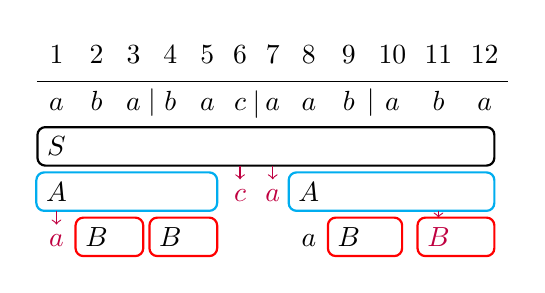
\begin{tikzpicture}
			\node[matrix of nodes, column sep=0mm, row sep=1mm, nodes in empty cells] (m) {
				$1$ & $2$ & $3$ & $4$ & $5$ & $6$ & $7$ & $8$ & $9$ & $10$ & $11$ & $12$\\\hline
        $a$ & $b$ & $a$ & $b$ & $a$ & $c$ & $a$ & $a$ & $b$ & $a$ & $b$ & $a$\\
				$S$ & & & & & & & & & & & \\
        $A$ & & & & & \textcolor{purple}{$c$} & \textcolor{purple}{$a$} & $A$ & & & & \\
        \textcolor{purple}{$a$} & $B$ & & $B$ & & & & $a$ & $B$ & & \textcolor{purple}{$B$} & \\
			};

			% Separators
			\node at ($(m-2-3)!0.5!(m-2-4)$) {$|$};
			\node at ($(m-2-6)!0.5!(m-2-7)$) {$|$};
			\node at ($(m-2-9)!0.5!(m-2-10)$) {$|$};

			\node[fit={(m-3-1.north west) (m-3-12.south east)},
				thick, inner sep=0, rounded corners=1mm,
				draw=black]{};

			\node[fit={(m-4-1.north west) (m-4-5.south east)},
				thick, inner sep=0, rounded corners=1mm,
				draw=cyan]{};
			\node[fit={(m-4-8.north west) (m-4-12.south east)},
				thick, inner sep=0, rounded corners=1mm,
				draw=cyan]{};

			\node[fit={(m-5-2.north west) (m-5-3.south east)},
				thick, inner sep=0, rounded corners=1mm,
				draw=red]{};
			\node[fit={(m-5-4.north west) (m-5-5.south east)},
				thick, inner sep=0, rounded corners=1mm,
				draw=red]{};
			\node[fit={(m-5-9.north west) (m-5-10.south east)},
				thick, inner sep=0, rounded corners=1mm,
				draw=red]{};
			\node[fit={(m-5-11.north west) (m-5-12.south east)},
				thick, inner sep=0, rounded corners=1mm,
				draw=red]{};

      \draw[->,purple] (m-4-1) -- (m-5-1);
      \draw[->,purple] (m-3-6) -- (m-4-6);
      \draw[->,purple] (m-3-7) -- (m-4-7);
      \draw[->,purple] (m-4-11) -- (m-5-11);
		\end{tikzpicture}
		\caption{Visual representation of the grammar.}
		\label{subfig:02:grammarvisual}
	\end{subfigure}
	\caption{An example of sampling with a grammar for the string $T = ababacaababa$. The chosen sampling rate is $r=3$.}
	\label{fig:02:samplingexample}
\end{figure}

\subsubsection{Queries}

Random access and substring queries follow the same general principle.
We choose the sample that lies in the same block as the query index.
From there, we scan until we have found the character or extracted all characters of the substring.

\paragraph{Random Access}

To answer a random access query for $1 \leq i \leq n$, we first determine the block $i$ is contained in, that being $k := \lceil i/r \rceil$.
Let $s_k =: (X, p_{\alpha}, p_{b_k}) \in (\mathcal{N} \cup \Sigma) \times \mathbb{N} \times \mathbb{N}$, where $\alpha$ is the right side of $X$. 
Then we know that $\alpha$ contains the character we are looking for since it spans the entire block $b_k$.
Depending on whether $i$ is lesser or greater than $k \cdot r + p_{b_k}$, we now just need to scan either backwards or forwards respectively,
descending into other nonterminals if necessary, in order to find the desired character.
While scanning we skip nonterminals that do not contain $i$ by making use of the saved length of the nonterminals' right side.

\paragraph{Substring}

Answering a substring query for $T[i..j]$ is similar to the random access query.
However, we answer a substring query block-wise. For each block that $T[i..j]$ spans we have a separate query.

For each of these queries we again find the correct sample $s_k$.
We then scan for the positions $i$ and $j$ and while doing so, instead of skipping non-terminals that do not contain $i$ and $j$
we return each terminal we encounter that is in $T[i..j]$.
This of course might require a forward \emph{and} backwards scan each block.

\section{Evaluation}

\todo{add evaluation results and describe them}

\section{Conclusion}

\printbibliography

\end{document}
